\documentclass[a4paper]{article}
\usepackage[utf8]{inputenc}
\usepackage[english]{babel}
\usepackage{graphicx}
\usepackage{hyperref}

\usepackage[
backend=biber,
sorting=none
]{biblatex}
\addbibresource{references.bib}

\begin{document}

\title{\Huge\textbf{MD5 Collision Attack Lab}\linebreak\linebreak\linebreak
\Large\textbf{Lab Report}\linebreak\linebreak
\linebreak\linebreak

\includegraphics[scale=0.1]{feup-logo.png}\linebreak\linebreak
\linebreak\linebreak
\Large{Integrated Master in Informatics and Computing Engineering} \linebreak\linebreak
\Large{Security in Computer Systems}\linebreak
}

\author{\textbf{Group 4:}\\
João Fidalgo - 201303098 \\
João Loureiro - 200806067 \\
Ka Chon Ho - 201711244 \\
Paulo Costa - 201206045 \\
\linebreak\linebreak
 \\ Faculdade de Engenharia da Universidade do Porto \\ Rua Roberto Frias, s\/n, 4200-465 Porto, Portugal \linebreak\linebreak\linebreak
\linebreak\linebreak\vspace{1cm}}

\maketitle

\newpage

\section{Introduction \cite{seed-labs}}

A secure one-way hash function needs to satisfy two properties: the one-way property and the collision-resistance property. The one-way property ensures that given a hash value $h$, it is computationally infeasible to find an input $M$, such that $hash(M) = h$. The collision-resistance property ensures that it is computationally infeasible to find two different inputs $M1$ and $M2$, such that $hash(M1) = hash(M2)$.

Several widely-used one-way hash functions have trouble maintaining the collision-resistance property. At the rump session of CRYPTO 2004, Xiaoyun Wang and co-authors demonstrated a collision attack against MD5 \cite{md5-col}. In February 2017, CWI Amsterdam and Google Research announced the SHAttered attack, which breaks the collision-resistance property of SHA-1 \cite{sha-1-col}. While many students do not have trouble understanding the importance of the one-way property, they cannot easily grasp why the collision-resistance property is necessary, and what impact these attacks can cause.

The learning objective of this lab is for students to really understand the impact of collision attacks, and see in first hand what damages can be caused if a widely-used one-way hash function’s collision-resistance property is broken. To achieve this goal, students need to launch actual collision attacks against the MD5 hash function. Using the attacks, students should be able to create two different programs that share the same MD5 hash but have completely different behaviors. This lab covers a number of topics described in the following:

\begin{itemize}
    \item One-way hash function
    \item The collision-resistance property
    \item Collision attacks
    \item MD5
\end{itemize}

\section{Setup}

The lab uses a tool called “Fast MD5 Collision Generation”, which was written by Marc Stevens; the name of the binary is called
\texttt{md5collgen} in our demonstration.

The result of the work of Marc Stevens et al as well as the source code of the \texttt{md5collgen} can be found at \href{https://www.win.tue.nl/hashclash}{https://www.win.tue.nl/hashclash}

To setup our machine we will need to download the source code for the \texttt{md5collgen}, install the dependencies and compile the code. The following steps are for a Debian like system such as Ubuntu.

Download the source code with the following command:

\bigskip

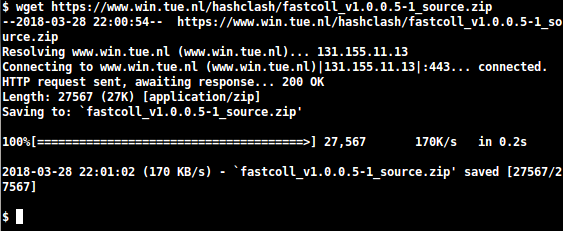
\includegraphics[width=0.9\textwidth]{bash/wget.png}

\bigskip

Then we need to extract the contents of the zip file we just downloaded.

\bigskip

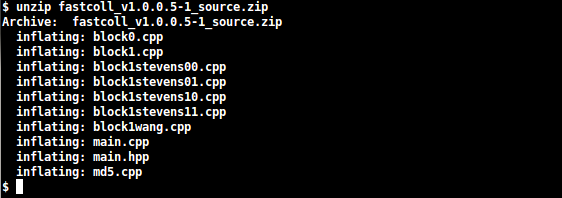
\includegraphics[width=0.9\textwidth]{bash/unzip.png}

\bigskip

Before we can compile the code we have extracted we need to install three boost libraries: \texttt{system}, \texttt{filesystem} and \texttt{program-options}.

\bigskip

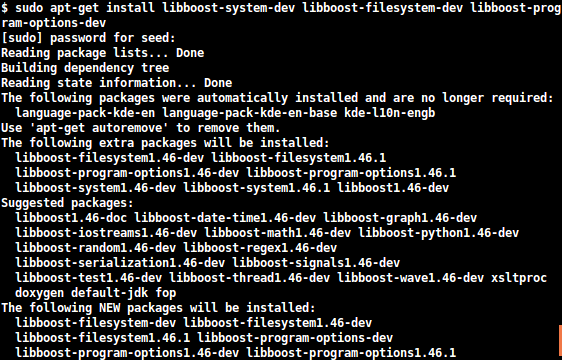
\includegraphics[width=0.9\textwidth]{bash/boost.png}

\bigskip

For the final step of our setup we need to compile the \texttt{md5collgen}.

\bigskip

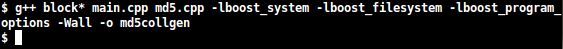
\includegraphics[width=0.9\textwidth]{bash/g++.png}

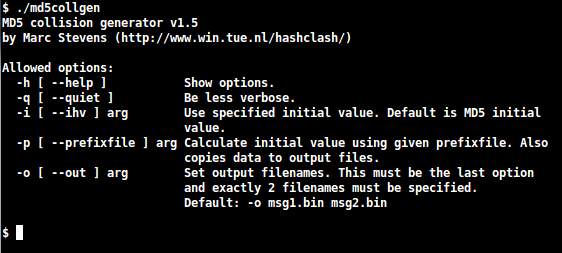
\includegraphics[width=0.9\textwidth]{bash/md5collgen.png}

\section{Lab Tasks}

\subsection{Task 1: Generating Two Different Files with the Same MD5 Hash}

In this task, we will generate two different files with the same MD5 hash values. The beginning parts of these two files need to be the same, i.e., they share the same prefix. We can achieve this using the \texttt{md5collgen} program, which allows us to provide a prefix file with any arbitrary content. The way how the program works is illustrated in Figure \ref{fig:md5gen}. The following command generates two output files, \texttt{out1.bin} and \texttt{out2.bin}, for a given a prefix file \texttt{prefix.txt}:

\begin{verbatim}
    $ md5collgen -p prefix.txt -o out1.bin out2.bin
\end{verbatim}

\begin{figure}[h]
    \centering
    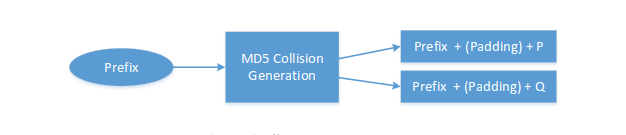
\includegraphics[width=\textwidth]{md5gen.png}
    \caption{MD5 collision generation from a prefix}
    \label{fig:md5gen}
\end{figure}

We can check whether the output files are distinct or not using the \texttt{diff} command. We can also use the \texttt{md5sum} command to check the MD5 hash of each output file. See the following commands.

\begin{verbatim}
    $ diff out1.bin out2.bin
    $ md5sum out1.bin
    $ md5sum out2.bin
\end{verbatim}

Since \texttt{out1.bin} and \texttt{out2.bin} are binary, we cannot view them using a text-viewer program, such as \texttt{cat} or \texttt{more}; we need to use a binary editor to view (and edit) them.

Please use such an editor to view these two output files, and describe your observations.

We first need to create a \texttt{prefix.txt} file. To be easy to detect that prefix in the binary file we created a \texttt{prefix.txt} with some A's, which translate to 41's in hex.

\bigskip

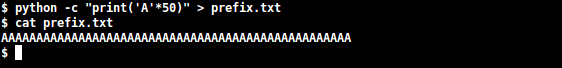
\includegraphics[width=0.9\textwidth]{bash/prefix.png}

\bigskip

After creating our \texttt{prefix.txt} we are now able to generate the two binaries with:

\bigskip

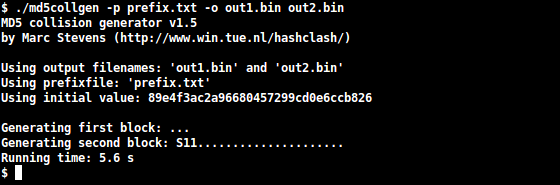
\includegraphics[width=0.9\textwidth]{bash/md5collgenout.png}

\bigskip

It generated the files quite fast, only 5.6 seconds. Now we are going to inspect if they are different but if they share the same hash.

\bigskip

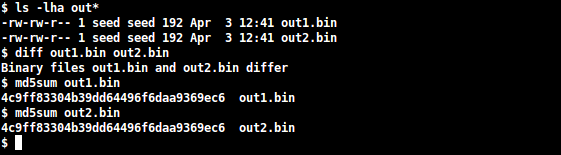
\includegraphics[width=0.9\textwidth]{bash/md5collgenoutcomp.png}

\bigskip

As we can see in the above image both files have the size of 192 bytes but they are different from each other and have the same MD5 hash. Which proves that MD5 is not collision-resistance and furthermore it is quite easy and quick to generate a collision.

If we look at what the program did with our prefix at the binary level.

\bigskip

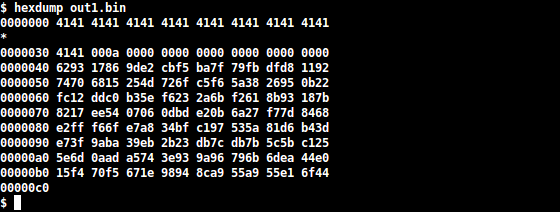
\includegraphics[width=0.9\textwidth]{bash/md5collgenoutdump.png}

\bigskip

The \texttt{md5collgen} took our \texttt{prefix.txt} added a new line at the end(0a) and filled 13 bytes with \texttt{NULL}(00). Our \texttt{prefix.txt} has 50 bytes(A's) if we add up the new line and the 13 \texttt{NULL}'s we end up with a magic number of 64 bytes that is equal to the size of a MD5 block. The size of the binaries is 192 bytes, if we subtract the 64 bytes of the prefix we know that 128 bytes of data was generated.

\bigskip

In addition, you should answer the following questions:

\textbf{Question 1.} If the length of your prefix file is not multiple of 64, what is going to happen?

\bigskip

We are going to create a \texttt{prefix.txt} with 64 A's and 10 B's (the B in hex is 42) and then we are going to generate the binaries.

\bigskip

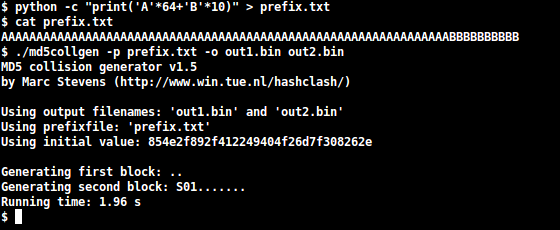
\includegraphics[width=0.9\textwidth]{bash/md5collgenoutAB.png}

\bigskip

If we \texttt{hexdump} one of the binaries we can see that it will fill until the next multiple of 64, that in this case is 128 bytes and generate the same 128 bytes of data.

\bigskip

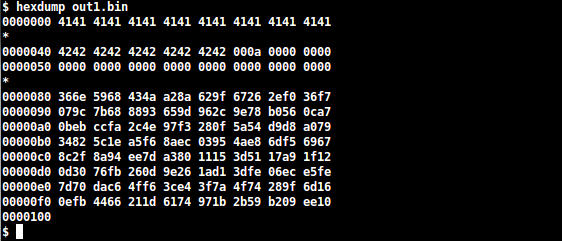
\includegraphics[width=0.9\textwidth]{bash/md5collgenoutdumpAB.png}

\newpage

\textbf{Question 2.} Create a prefix file with exactly 64 bytes, and run the collision tool again, and see what happens.

\bigskip

If the \texttt{prefix.txt} is exactly 64 bytes the program will add a new line and 63 \texttt{NULL}'s making a total of 128 bytes, same as the example before.

\bigskip

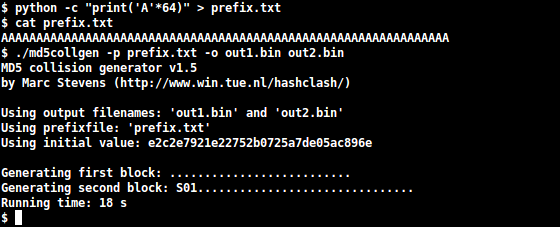
\includegraphics[width=0.9\textwidth]{bash/md5collgenout64.png}

\bigskip

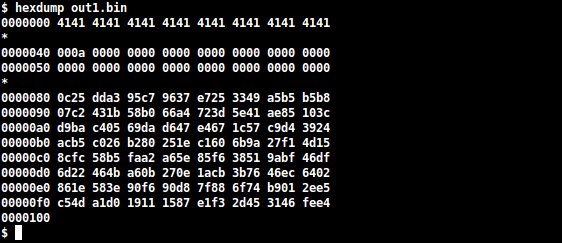
\includegraphics[width=0.9\textwidth]{bash/md5collgenoutdump64.png}

\bigskip

\textbf{Question 3.} Are the data (128 bytes) generated by \texttt{md5collgen} completely different for the two output files? Please identify all the bytes that are different

\bigskip

Storing the hex representation of the binaries into a file and then comparing the two we can see that they are not that different, in fact they only differ in the first 4 bits of 4 bytes.

\bigskip

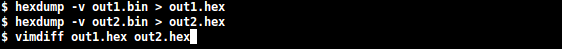
\includegraphics[width=0.9\textwidth]{bash/md5collgenoutdumpfile.png}

\bigskip

\bigskip

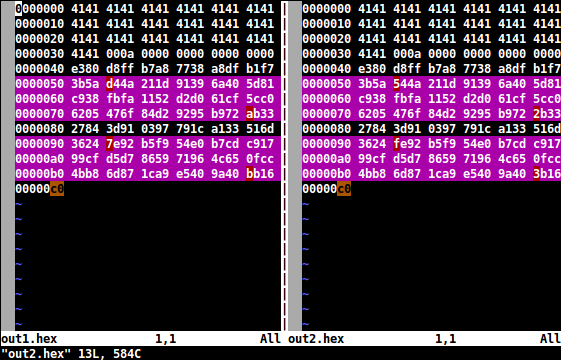
\includegraphics[width=0.9\textwidth]{bash/md5collgenoutdumpvimdiff.png}

\bigskip

\subsection{Task 2: Understanding MD5’s Property}

In this task, we will try to understand some of the properties of the MD5 algorithm. These properties are important for us to conduct further tasks in this lab. MD5 is a quite complicated algorithm, but from very high level, it is not so complicated. As Figure \ref{fig:md5ihv} shows, MD5 divides the input data into blocks of 64 bytes, and then computes the hash iteratively on these blocks. The core of the MD5 algorithm is a compression function, which takes two inputs, a 64-byte data block and the outcome of the previous iteration. The compression function produces a 128-bit IHV, which stands for “Intermediate Hash Value”; this output is then fed into the next iteration. If the current iteration is the last one, the IHV will be the final hash value. The IHV input for the first iteration (IHV$_0$) is a fixed value,

\begin{figure}[h]
    \centering
    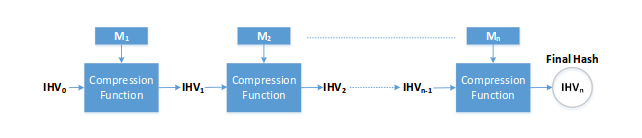
\includegraphics[width=\textwidth]{md5ihv.png}
    \caption{How the MD5 algorithm works}
    \label{fig:md5ihv}
\end{figure}

Based on how MD5 works, we can derive the following property of the MD5 algorithm: Given two inputs $M$ and $N$, if $MD5(M) = MD5(N)$, i.e., the MD5 hashes of $M$ and $N$ are the same, then for any input $T$, $MD5(M || T) = MD5(N || T)$, where $||$ represents concatenation. That is, if inputs $M$ and $N$ have the same hash, adding the same suffix $T$ to them will result in two outputs that have the same hash value. This property holds not only for the MD5 hash algorithm, but also for many other hash algorithms. Your job in this task is to design an experiment to demonstrates that this property holds for MD5. You can use the \texttt{cat} command to concatenate two files (binary or text files) into one. The following command concatenates the contents of \texttt{file2} to the contents of \texttt{file1} , and places the result in \texttt{file3}.

\begin{verbatim}
    $ cat file1 file2 > file3
\end{verbatim}

The two binaries that have the same hash but differ from each other will be used to demonstrate this MD5 property.

\bigskip

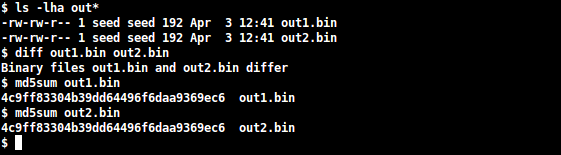
\includegraphics[width=0.9\textwidth]{bash/md5collgenoutcomp.png}

\bigskip

If we create a \texttt{suffix.txt} file concatenate it with our binaries to another file and compare the new MD5 hashes of the two new generated files we can verify they are the same.

\bigskip

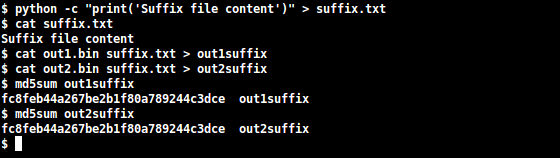
\includegraphics[width=0.9\textwidth]{bash/md5suffix.png}

\bigskip

\subsection{Task 3: Generating Two Executable Files with the Same MD5 Hash}

In this task, you are given the following C program. Your job is to create two different versions of this program, such that the contents of their \texttt{xyz} arrays are different, but the hash values of the their executables are the same.

\begin{verbatim}
    #include <stdio.h>
    unsigned char xyz[200] = {
    /
    *
    The actual contents of this array are up to you
    *
    /
    };
    int main()
    {
        int i;
        for (i=0; i<200; i++){
            printf("%x", xyz[i]);
        }
        printf("\n");
    }
\end{verbatim}

You may choose to work at the source code level, i.e., generating two versions of the above C program, such that after compilation, their corresponding executable files have the same MD5 hash value. However, it may be easier to directly work on the binary level. You can put some random values in the \texttt{xyz} array, compile the above code to binary. Then you can use a hex editor tool to modify the content of the \texttt{xyz} array directly in the binary file.

Finding where the contents of the array are stored in the binary is not easy. However, if we fill the array with some fixed values, we can easily find them in the binary. For example, the following code fills the array with \texttt{0x41}, which is the ASCII value for letter A. It will not be difficult to locate 200 \texttt{A}’s in the binary.

\begin{verbatim}
    unsigned char xyz[200] = {
    0x41, 0x41, 0x41, 0x41, 0x41, 0x41, 0x41, 0x41, 0x41, 0x41,
    0x41, 0x41, 0x41, 0x41, 0x41, 0x41, 0x41, 0x41, 0x41, 0x41,
    0x41, 0x41, 0x41, 0x41, 0x41, 0x41, 0x41, 0x41, 0x41, 0x41,
    ... (omitted) ...
    0x41, 0x41, 0x41, 0x41, 0x41, 0x41, 0x41, 0x41, 0x41, 0x41
    }
\end{verbatim}

\textbf{Guidelines} From inside the array, we can find two locations, from where we can divide the executable file into three parts: a prefix, a 128-byte region, and a suffix. The length of the prefix needs to be multiple of 64 bytes. See Figure \ref{fig:preffixsuffix} for an illustration of how the file is divided.

\begin{figure}[h]
    \centering
    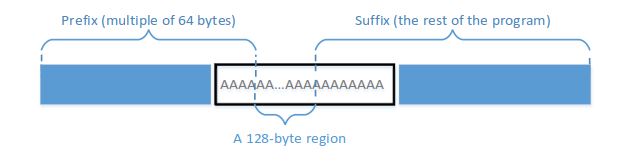
\includegraphics[width=\textwidth]{prefixsuffix.png}
    \caption{Break the executable file into three pieces.}
    \label{fig:preffixsuffix}
\end{figure}

We can run \texttt{md5collgen} on the prefix to generate two outputs that have the same MD5 hash value. Let us use \texttt{P} and \texttt{Q} to represent the second part (each having 128 bytes) of these outputs (i.e., the part after the prefix). Therefore, we have the following:

\bigskip

$MD5 (prefix || P) = MD5 (prefix || Q)$

\bigskip

Based on the property of MD5, we know that if we append the same suffix to the above two outputs, the resultant data will also have the same hash value. Basically, the following is true for any suffix:

\bigskip

$MD5 (prefix || P || suffix) = MD5 (prefix || Q || suffix)$

\bigskip

Therefore, we just need to use \texttt{P} and \texttt{Q} to replace 128 bytes of the array (between the two dividing points), and we will be able to create two binary programs that have the same hash value. Their outcomes are different, because they each print out their own arrays, which have different contents.

\textbf{Tools} You can use \texttt{bless} to view the binary executable file and find the location for the array. For dividing a binary file, there are some tools that we can use to divide a file from a particular location. The \texttt{head} and \texttt{tail} commands are such useful tools. You can look at their manuals to learn how to use them. We give three examples in the following:

\begin{verbatim}
    $ head -c 3200 a.out > prefix
    $ tail -c 100 a.out > suffix
    $ tail -c +3300 a.out > suffix
\end{verbatim}

The first command above saves the first \texttt{3200} bytes of \texttt{a.out} to \texttt{prefix}. The second command saves the last \texttt{100} bytes of \texttt{a.out} to \texttt{suffix}. The third command saves the data from the \texttt{3300}th byte to the end of the file \texttt{a.out} to \texttt{suffix}. With these two commands, we can divide a binary file into pieces from any location. If we need to glue some pieces together, we can use the \texttt{cat} command.

\bigskip

First we will create a file named \texttt{md5coll.c} with the following C code.

\bigskip

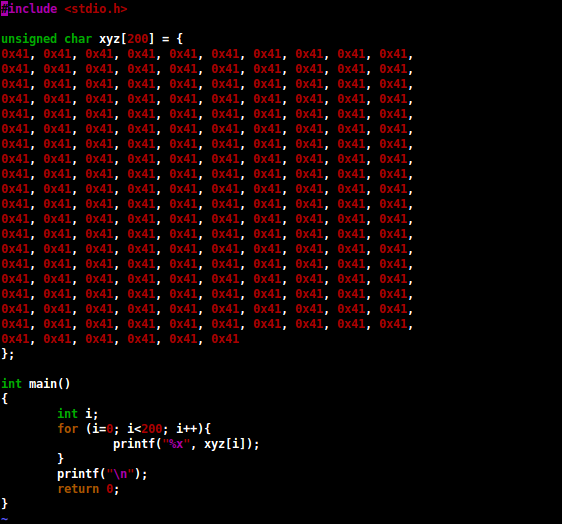
\includegraphics[width=0.9\textwidth]{bash/md5coll.png}

\bigskip

After that we need to compile the code using the gcc compiler.

\bigskip

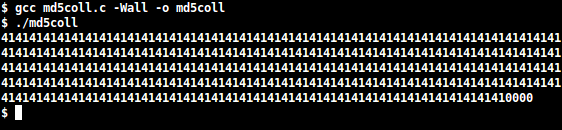
\includegraphics[width=0.9\textwidth]{bash/md5collgcc.png}

\bigskip

Now that we have the binary \texttt{md5coll}, we need to search for the 200 A's that we have in the array. We can do that by running the following command and searching for the hex representation of A which is 41.

\begin{verbatim}
    $ hexdump -v md5coll
\end{verbatim}

\bigskip

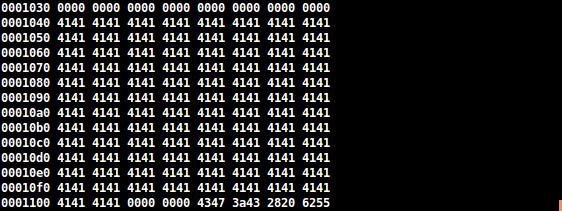
\includegraphics[width=0.9\textwidth]{bash/md5colldump.png}

\bigskip

We can see in the image above that the array starts at the position \texttt{1040} in decimal it's \texttt{4160} bytes. We know that the array size is \texttt{200 bytes} so now we just need to extract the first \texttt{4160} bytes for the prefix and from the \texttt{4260} byte forward.

\bigskip

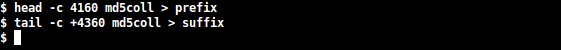
\includegraphics[width=0.9\textwidth]{bash/md5collcrop.png}

\bigskip

Now we use our \texttt{md5collgen} program with the prefix to generate two different outputs with the same MD5 hash.

\bigskip

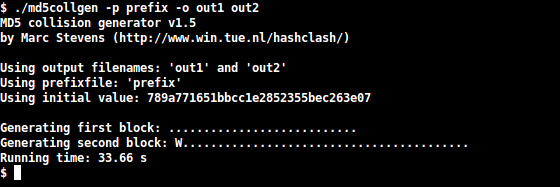
\includegraphics[width=0.9\textwidth]{bash/md5collgenerate.png}

\bigskip

Using the properties of the MD5 algorithm we now concatenate the two diferent outputs of the \texttt{md5collgen} program with the suffix and the hash will remain the same.

\bigskip

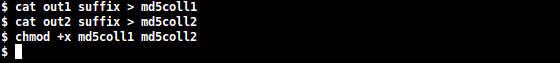
\includegraphics[width=0.9\textwidth]{bash/md5collcat.png}

\bigskip

Now as we can see bellow the two programs \texttt{md5coll1} and \texttt{md5coll2} are different but share the same hash.

\bigskip

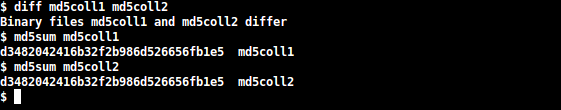
\includegraphics[width=0.9\textwidth]{bash/md5colldiff.png}

\bigskip

We only need to run both programs and check if they run and if the outputs differ, and they do.

\bigskip

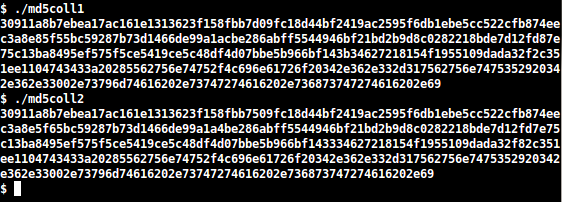
\includegraphics[width=0.9\textwidth]{bash/md5collexec.png}

\bigskip

\newpage

\subsection{Task 4: Making the Two Programs Behave Differently}

In the previous task, we have successfully created two programs that have the same MD5 hash, but their behaviors are different. However, their differences are only in the data they print out; they still execute the same sequence of instructions. In this task, we would like to achieve something more significant and more meaningful.

Assume that you have created a software which does good things. You send the software to a trusted authority to get certified. The authority conducts a comprehensive testing of your software, and concludes that your software is indeed doing good things. The authority will present you with a certificate, stating that your program is good. To prevent you from changing your program after getting the certificate, the MD5 hash value of your program is also included in the certificate; the certificate is signed by the authority, so you cannot change anything on the certificate or your program without rendering the signature invalid.

You would like to get your malicious software certified by the authority, but you have zero chance to achieve that goal if you simply send your malicious software to the authority. However, you have noticed that the authority uses MD5 to generate the hash value. You got an idea. You plan to prepare two different programs. One program will always execute benign instructions and do good things, while the other program will execute malicious instructions and cause damages. You find a way to get these two programs to share the same MD5 hash value.

You then send the benign version to the authority for certification. Since this version does good things, it will pass the certification, and you will get a certificate that contains the hash value of your benign program. Because your malicious program has the same hash value, this certificate is also valid for your malicious program. Therefore, you have successfully obtained a valid certificate for your malicious program. If other people trusted the certificate issued by the authority, they will download your malicious program.

The objective of this task is to launch the attack described above. Namely, you need to create two programs that share the same MD5 hash. However, one program will always execute benign instructions, while the other program will execute malicious instructions. In your work, what benign/malicious instructions are executed is not important; it is sufficient to demonstrate that the instructions executed by these two programs are different.

\textbf{Guidelines} Creating two completely different programs that produce the same MD5 hash value is quite hard. The two hash-colliding programs produced by \texttt{md5collgen} need to share the same prefix; moreover, as we can see from the previous task, if we need to add some meaningful suffix to the outputs produced by \texttt{md5collgen}, the suffix added to both programs also needs to be the same. These are the limitations of the MD5 collision generation program that we use. Although there are other more complicated and more advanced tools that can lift some of the limitations, such as accepting two different prefixes [2], they demand much more computing power, so they are out of the scope for this lab. We need to find a way to generate two different programs within the limitations.

There are many ways to achieve the above goal. We provide one approach as a reference, but students are encouraged to come up their own ideas. Instructors may consider rewarding students for their own ideas. In our approach, we create two arrays \texttt{X} and \texttt{Y}. We compare the contents of these two arrays; if they are the same, the benign code is executed; otherwise, the malicious code is executed. See the following pseudo-code:

\begin{verbatim}
    Array X;
    Array Y;
    main()
    {
        if(X’s contents and Y’s contents are the same)
            run benign code;
        else
            run malicious code;
        return;
    }
\end{verbatim}

We can initialize the arrays \texttt{X} and \texttt{Y} with some values that can help us find their locations in the executable binary file. Our job is to change the contents of these two arrays, so we can generate two different versions that have the same MD5 hash. In one version, the contents of \texttt{X} and \texttt{Y} are the same, so the benign code is executed; in the other version, the contents of \texttt{X} and \texttt{Y} are different, so the malicious code is executed. We can achieve this goal using a technique similar to the one used in Task 3. Figure \ref{fig:behaviorprog} illustrates what the two versions of the program look like.

\begin{figure}[h]
    \centering
    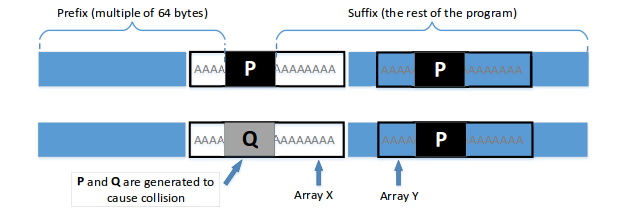
\includegraphics[width=\textwidth]{behaviorprog.png}
    \caption{An approach to generate two hash-colliding programs with different behaviors.}
    \label{fig:behaviorprog}
\end{figure}

From Figure \ref{fig:behaviorprog}, we know that these two binary files have the same MD5 hash value, as long as \texttt{P} and \texttt{Q} are generated accordingly. In the first version, we make the contents of arrays \texttt{X} and \texttt{y} the same, while in the second version, we make their contents different. Therefore, the only thing we need to change is the contents of these two arrays, and there is no need to change the logic of the programs.

\bigskip

First we need to write the code of the program, it will be something like the following.

\bigskip

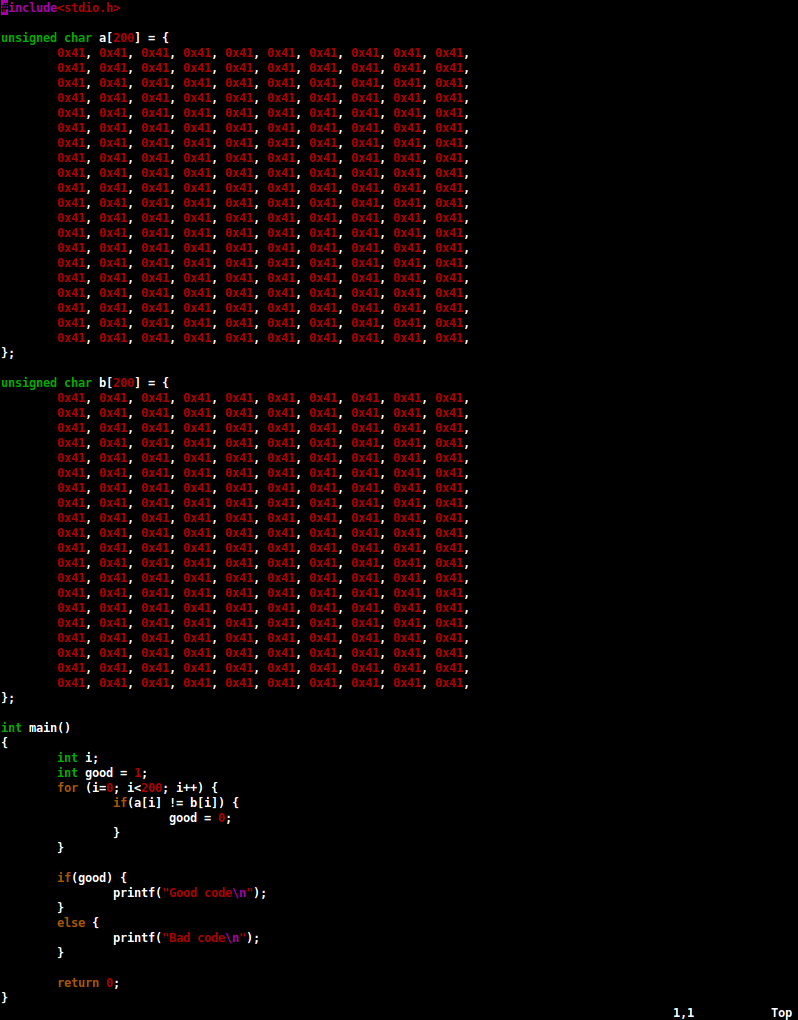
\includegraphics[width=0.7\textwidth]{bash/md5collarray.png}

\bigskip

In the above code we have to \texttt{char} array's with 200 \texttt{A}'s each. We then compare the two arrays and if they are equal we execute good code if they are not we execute bad code. Now we need to compile the code into a binary file.

\bigskip

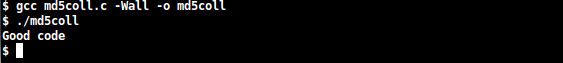
\includegraphics[width=0.9\textwidth]{bash/md5collarraygcc.png}

As expected, because the two array's are equal we have good code as the output. Now we need to take a look at our binary using \texttt{hexdump}.

\bigskip

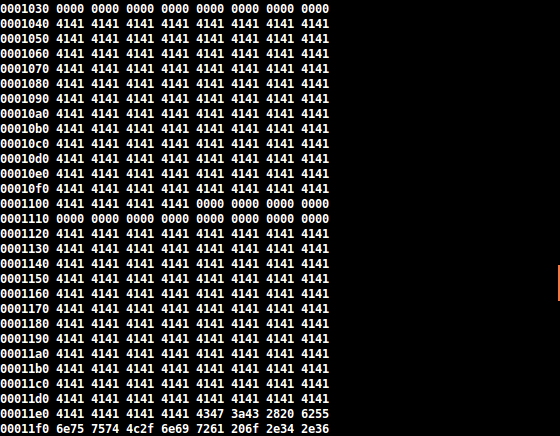
\includegraphics[width=0.9\textwidth]{bash/md5collarraydump.png}

\bigskip

We can see in the image above that we have the beginning of the first array at the position \texttt{1040} in other words we have \texttt{0x1040 = 4160 bytes} before the first array. We the have \texttt{24 bytes} of \texttt{NULL}'s and then the second array ending at \texttt{0x11e8 = 4584 bytes}, which means rest of the program is from the \texttt{byte 4585} forward. With that information we can create a prefix and a suffix.

\bigskip

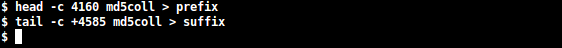
\includegraphics[width=0.9\textwidth]{bash/md5collarraypresuf.png}

\bigskip

Now that we have a prefix we can create two different files with the same MD5 hash with the \texttt{md5collgen} program as seen before.

\bigskip

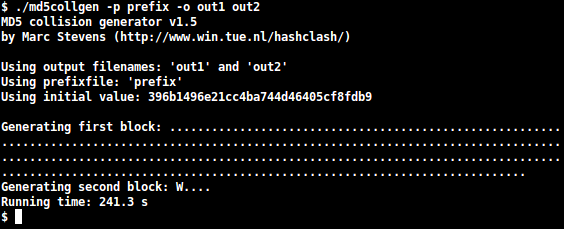
\includegraphics[width=0.9\textwidth]{bash/md5collarraygenerate.png}

\bigskip

From our previous experiments we know that \texttt{md5collgen} generates \texttt{128 bytes} of data, see the image below that contains the \texttt{hexdump} of \texttt{out1}. The arrays that we have are \texttt{200 bytes} long so we need to fill the remaining \texttt{72 bytes}, then we need to add those \texttt{24 bytes} of \texttt{NULL}'s that we have seen before. For the second array, in both cases we need to add the \texttt{128 bytes} of generated data from \texttt{out1} and fill the remainder \texttt{72 bytes}.

\bigskip

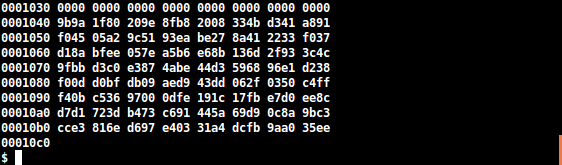
\includegraphics[width=0.9\textwidth]{bash/md5collarrayoutdump.png}

\bigskip

For those reasons we create three files: array, that contains the \texttt{128 bytes} of data from \texttt{out1}; padding, that contains the \texttt{24 bytes} of \texttt{NULL}'s; and fill, that contains \texttt{72 bytes} of filling(\texttt{A}'s in this case).

\bigskip

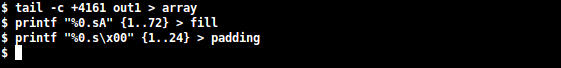
\includegraphics[width=0.9\textwidth]{bash/md5collarrayoutarray.png}

\bigskip

Now we use \texttt{out1}, \texttt{out2}, \texttt{fill}, \texttt{padding}, \texttt{array} and \texttt{suffix} to build two binaries, one that runs good code and another that runs bad code but share the same MD5 hash.

\bigskip

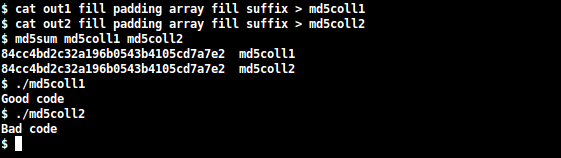
\includegraphics[width=0.9\textwidth]{bash/md5collarraycat.png}

\bigskip

It's noticeable that one ill-intended person with sufficient time and cunning can use this process to do a great deal of damage in real world systems that still rely on the MD5 algorithm. The work of Marc Stevens makes it extremely easy to generate data that shares the same MD5 hash.

\newpage

\printbibliography

\end{document}

